% !TEX root = ../../main.tex

\section{Materials and characterisation methods}

\subsection{Materials}

Several DUT materials have been synthesised in order to 
study the effect of different parameters on the switching 
behaviour. From the point of view of the criterion of interest,
the materials can be divided into the following categories:

\begin{itemize}
    \item Series dedicated to studying the influence of isoreticular
    design through variation of linker length in the order of 
    theoretical increasing porosity: DUT-48, DUT-46, DUT-49, 
    DUT-50, DUT-151/DUT-152. These materials are designed 
    with a linker of increasing size by using differently 
    structured phenyl rings. A corresponding increase in 
    porosity is expected, however, starting from a 4-linear
    phenyl chain (DUT-151), the internal voids are large enough to 
    allow for a secondary interpenetrated network to develop.
    An attempt to prevent this by grafting bulky naphthalene 
    rings was made in the synthesis of DUT-152, but the resulting 
    structure was still found to be interpenetrated.
    
    \item Series assessing the impact of steric hindrance of the 
    central linker bond on NGA, in the order of connectivity:
    DUT-49, DUT-149, DUT-148, DUT-147. The rationale behind this
    approach is to improve the tensile strength of the strut by 
    the addition of sterically hindering side connections.

    \item Series investigating the effect of heterocycles on compliant
    behaviour, using thiophene as replacement for the benzene rings, 
    in the order of increasing linker size: DUT-170, DUT-171, DUT-172,
    DUT-173. If interactions with the framework plays a role in NGA,
    the addition of potentially stronger host-guest sites.

    \item Series aiming to possess a progressively more labile central 
    strut through the use of different degrees of saturation,
    in order of central bond hybridization: DUT-160, DUT-161, DUT-163.
    It was found that the removal of solvent from DUT-162 could not be 
    performed without structure collapse. The softness of the saturated
    backbone lends itself to an unstable \textit{op} state.

    \item Series of increasing crystallite size to study the effect 
    of the crystal surface to volume ratio on NGA. Different sizes
    of DUT-49 were synthesised either through the addition of a 
    acid modulator for obtaining large crystals or through the addition
    of a base to inhibit crystal growth. A series of 4 DUT-49 
    was received, of \SI{800}{\nano\metre}, \SI{1}{\micro\metre},
    \SI{4}{\micro\metre} and \SI{10}{\micro\metre} average size 
    respectively.

\end{itemize}

\todo{Need data from simon on these materials}

The material name, together with the central part of the linker, 
which was modified to change the flexible behaviour of the framework,
is presented in \autoref{dut:tab:materials}.

\begin{table}[p]
    \centering %
	\caption{Flexible materials analogous to DUT-49}
    \small
    \begin{tabular}{c >{\centering}m{6cm} c p{4cm}}
		\toprule
	    \textbf{Name}
        & \textbf{Linker center}
        & \textbf{Study}
        & \textbf{Observations} \\
		\midrule
        DUT-49  & 
            
\includegraphics[width=4cm]{structures/DUT-49}
            & Original material & 
            \makecell[l]{
            Multiple crystal sizes \\ %
            \scriptsize\llap{\textbullet}~~DUT-49(o)-\SI{0.8}{\micro\metre}\\%
            \scriptsize\llap{\textbullet}~~DUT-49(s)-\SI{1.0}{\micro\metre}\\%
            \scriptsize\llap{\textbullet}~~DUT-49(m)-\SI{4.0}{\micro\metre}\\%
            \scriptsize\llap{\textbullet}~~DUT-49(l)-\SI{10.0}{\micro\metre}} \\
        \midrule
        DUT-48  & 
            
\includegraphics[width=2.5cm]{structures/DUT-48}
            & Linker size & --- \\
        DUT-46  & 
            
\includegraphics[width=3cm]{structures/DUT-46}
            & Linker size & --- \\
        DUT-50  & 
            
\includegraphics[width=5.3cm]{structures/DUT-50}
            & Linker size & --- \\
        DUT-151  & 
            
\includegraphics[width=5cm]{structures/DUT-151} 
            & Linker size & Interpenetrated \\
        DUT-152  & 
            
\includegraphics[width=5cm]{structures/DUT-152}
            & Linker size & Interpenetrated \\
            \midrule
        DUT-149  & 
            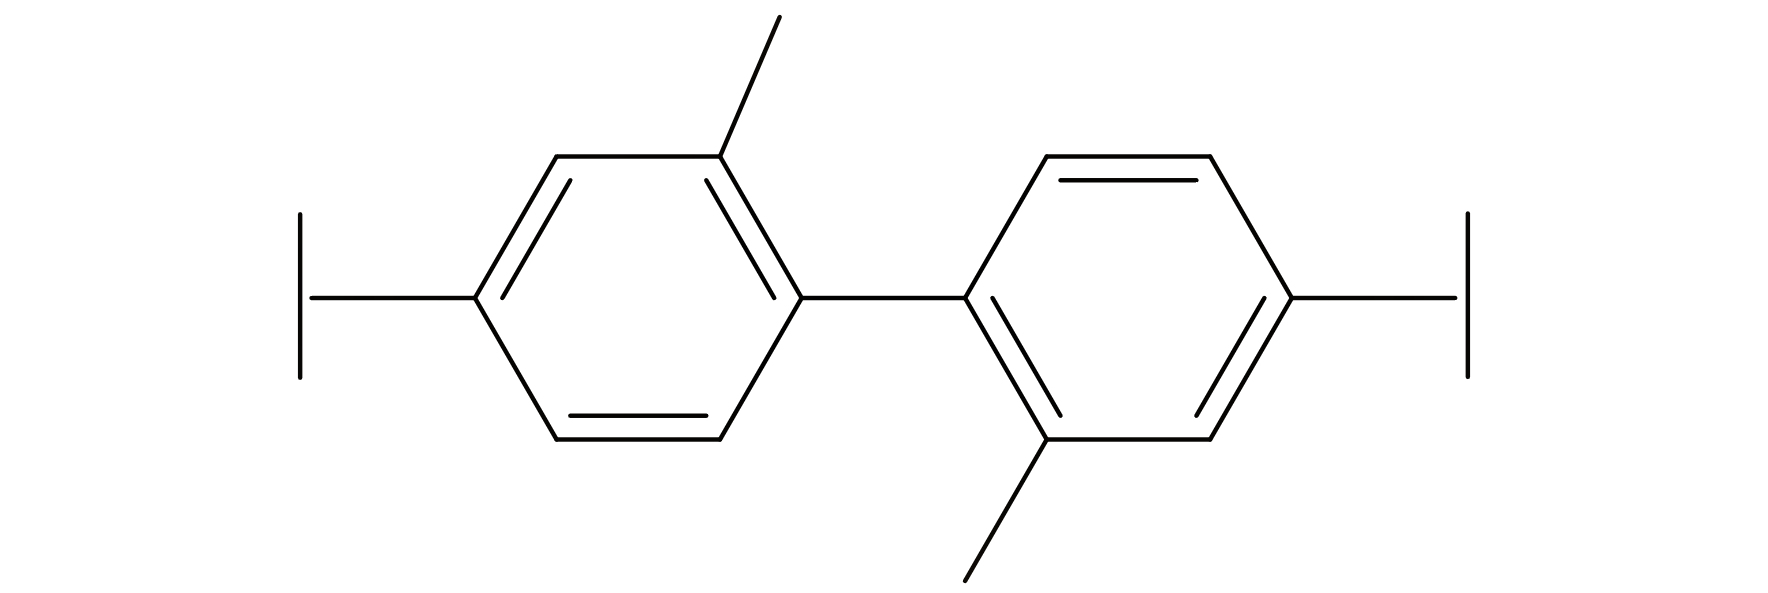
\includegraphics[width=3.8cm]{structures/DUT-149}
            & Functionalization & --- \\
        DUT-148  & 
            
\includegraphics[width=3.8cm]{structures/DUT-148}
            & Functionalization & --- \\
        DUT-147  & 
            
\includegraphics[width=3.8cm]{structures/DUT-147}
            & Functionalization & --- \\
            \midrule
            DUT-170  & 
            
\includegraphics[width=3.2cm]{structures/DUT-170}
            & Heterocycle & --- \\
            DUT-171  & 
            
\includegraphics[width=4cm]{structures/DUT-171}
            & Heterocycle & --- \\
            DUT-172  & 
            
\includegraphics[width=4cm]{structures/DUT-172}
            & Heterocycle & Not measured \\
            DUT-173  & 
            
\includegraphics[width=5.5cm]{structures/DUT-173}
            & Heterocycle & Not measured \\
        \midrule
        DUT-160  & 
            
\includegraphics[width=5cm]{structures/DUT-160}
            & Strut saturation & --- \\
        DUT-161  & 
            
\includegraphics[width=5cm]{structures/DUT-161}
            & Strut saturation & Not measured \\
        DUT-162  & 
            
\includegraphics[width=5cm]{structures/DUT-162}
            & Strut saturation & No stable \textit{op} state \\
        \bottomrule
	\end{tabular}%
	\label{dut:tab:materials}
\end{table}%

\subsection{Characterisation methods}

In order to examine the energetic components of both adsorption and 
NGA, the combined manometry and calorimetry setup first 
presented in \autoref{calo} was used. Ambient temperature calorimetry
was conducted at \SI{303}{\kelvin} with probes such as butane, propane
and propylene using the step-by-step gas introduction method. 
The exact procedure for such an experiment can be found in 
\autoref{appx:char:ambient-calo} of \autoref{appx:char}.

For low temperatures (\SI{77}{\kelvin}), a high resolution continuous
introduction method was employed, together with a home-made 
calorimetric system first described in the work 
of~\citet{rouquerolCalorimetricEvidenceBidimensional1977}. To summarize,
the adsorbate is placed in a J-shaped custom designed glass cell which is
then sealed with an oxyacetylene torch prior to evacuation and sample 
activation. Borosilicate glass is selected as
the material of choice to prevent any thermal expansion induced leaks.
The cell is then introduced into a \ce{LN2}-filled dewar, through 
the bottom of the differential calorimeter. Good thermal equilibrium
between the cell and surrounding thermopile is ensured using by 
using a helium blanket in the calorimetric enclosure, kept under 
positive pressure through a continuous low flow. The connection to the 
gas dosing system is made through a Swagelock VCR \(\sfrac{1}{4}''\)
stainless steel connection. High leak resistance and gas purity 
is assured by the single use copper joint metal-to-metal interlock.
Pressure is measured through the use of a double gauge assembly,
a sensitive low pressure gauge (up to \SI{2}{\kilo\pascal}) and 
an ambient pressure gauge (up to \SI{120}{\kilo\pascal}).
A sonic nozzle is used to control the flow of adsorbate into the 
reference volume and the cell. A separate calibration step is 
performed at the start of each experiment to determine the adsorbate
flowrate and the dead volume before the entrance to the cell.
An experiment takes between 1--4 days depending 
on the flowrate used. A picture of the different components of the 
setup can be seen in \autoref{dut:fgr:ltc-setup}.

\begin{figure}[htb]
    \centering
    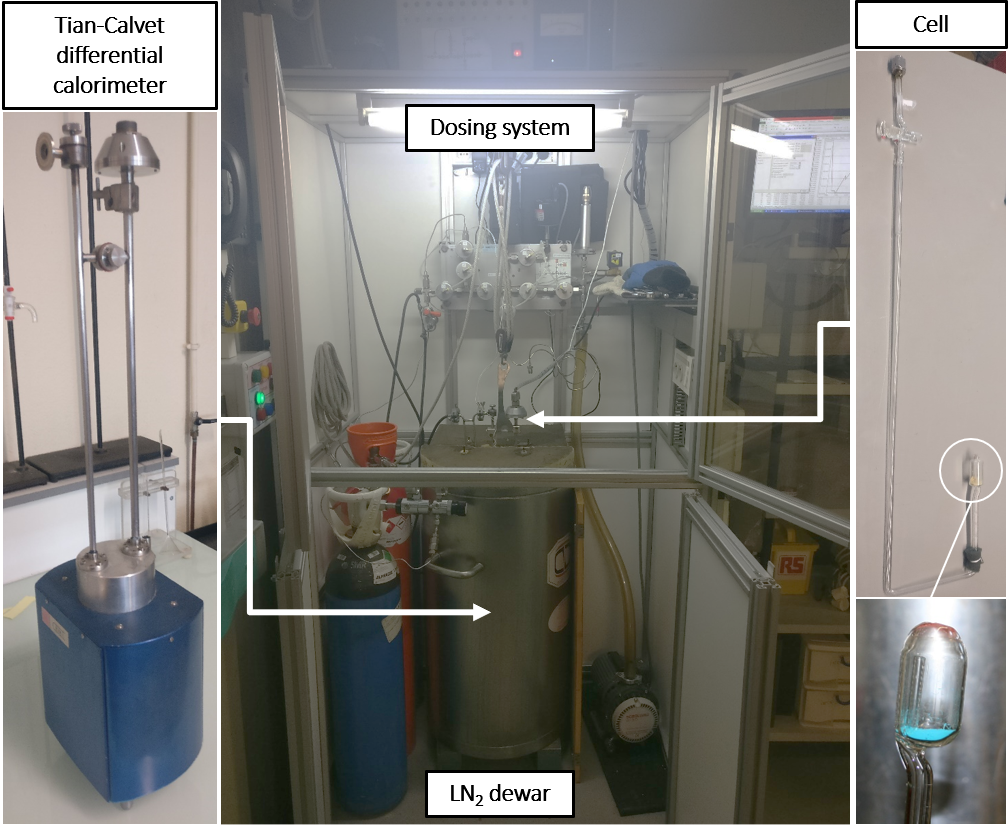
\includegraphics[width=0.9\textwidth]{ltc-setup}%
    \caption{The low temperature calorimetry setup}%
    \label{dut:fgr:ltc-setup}
\end{figure}

Extreme care has to be taken during sample preparation, as all materials 
studied are sensitive to heat and water vapour, which attack
the Cu paddlewheel and lead to material degradation. To prevent any 
decomposition, the samples were stored under an inert argon 
atmosphere in a glovebox. The loading of ambient temperature 
cells was performed inside the glovebox while filling and sealing 
of low temperature glass cells was done in an argon flow. After 
sample cell preparation, the materials are activated under 
dynamic vacuum at \SI{120}{\degreeCelsius}. 

It is worth noting that if the sample undergoes an \textit{op}/\textit{cp}
phase transition during the experiment and cannot be reopened with
the application of high pressure, as is the case for butane at 
\SI{303}{\kelvin}, the material cannot be reused. Any attempt to
activate it under vacuum leads to structural breakdown of the 
unstable \textit{cp} phase. 
Since a limited amount of sample is available, this played a large
role in data acquisition, with several isotherms only recorded once.
